\documentclass[tikz,border=8pt]{standalone}
\usetikzlibrary{arrows.meta,positioning}
\begin{document}
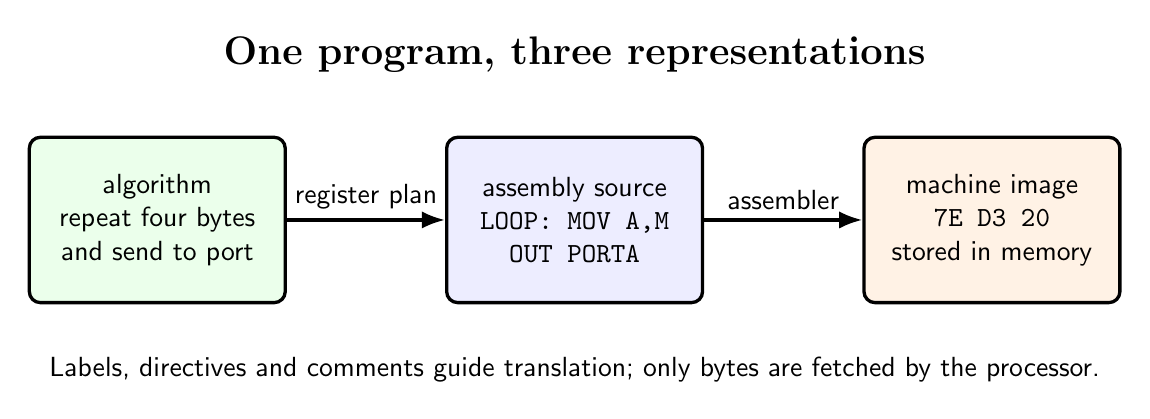
\begin{tikzpicture}[font=\sffamily,>=Latex,
  box/.style={draw,very thick,rounded corners,minimum width=3.25cm,minimum height=2.1cm,align=center}]
\node[font=\Large\bfseries] at (7.1,4.35) {One program, three representations};
\node[box,fill=green!8] (alg) at (1.8,2.25) {algorithm\\repeat four bytes\\and send to port};
\node[box,fill=blue!7] (src) at (7.1,2.25) {assembly source\\\texttt{LOOP: MOV A,M}\\\texttt{OUT PORTA}};
\node[box,fill=orange!10] (obj) at (12.4,2.25) {machine image\\\texttt{7E D3 20}\\stored in memory};
\draw[very thick,->] (alg)-- node[above] {register plan} (src);
\draw[very thick,->] (src)-- node[above] {assembler} (obj);
\node[align=center] at (7.1,.35) {Labels, directives and comments guide translation; only bytes are fetched by the processor.};
\end{tikzpicture}
\end{document}
